\documentclass[conference]{IEEEtran}
\usepackage[T1]{fontenc}
\usepackage{graphicx}
\usepackage{booktabs}
\usepackage{amsmath}
\usepackage{url}
\usepackage{cite}
\usepackage[hidelinks]{hyperref}
\graphicspath{{figs/}}

\begin{document}

\title{An Open, Low-Cost Prototype for AI-Assisted Heart and Lung Auscultation with Patient Intake and Doctor Handoff}

\author{\IEEEauthorblockN{Aditya Vardhan}
\IEEEauthorblockA{University of Roehampton\\London, United Kingdom}}

\maketitle

\begin{abstract}
Stethoscope findings depend on the listener, and many clinicians in primary care have little time to listen carefully. This report describes a working research prototype that analyses heart and lung sound recordings, combines the two into one report, and passes a structured patient summary to a doctor. Five classifiers were trained only on free public datasets (PhysioNet/CinC 2016, CirCor DigiScope, Yaseen 2018, ICBHI 2017 and KAUH 2021), with every test set held out by patient wherever the data allowed it. On held-out data the adult heart model reaches a mean accuracy (MAcc) of 0.882, the paediatric murmur model 0.724, and the four-class lung sound model an ICBHI score of 0.508, below the published state of the art of about 0.60 to 0.65. An outlier detector rejects audio that does not resemble a stethoscope recording, and a transparent rule layer adds cross-system flags such as murmur with crackles. The system runs as a FastAPI service and a phone web app on a free hosting tier; in a live check, 32 of 34 held-out samples matched their dataset labels, with a median response time of 1.6~s. Four attempts to improve the lung model were evaluated: an ImageNet-pretrained CNN, a CNN plus boosting ensemble, frozen AudioSet-pretrained transformer (AST) embeddings (0.533) and a slimmed int8 AST that runs ten times faster (0.519). A patient-level bootstrap shows none of these gains is statistically clear on a 49-patient test set, so the boosting model stays in production. The report closes with the work still needed before clinical use: fine-tuned lung models, a real digital stethoscope, an NHS pilot, and the UK regulatory route for software as a medical device.
\end{abstract}

\begin{IEEEkeywords}
auscultation, heart sound, lung sound, phonocardiogram, machine learning, LightGBM, audio spectrogram transformer, decision support, telemedicine, NHS
\end{IEEEkeywords}

\section{Introduction}
Auscultation is cheap and fast, but it is also subjective. Murmurs, crackles and wheezes are easy to miss in a noisy room, and the skill fades without practice. Digital stethoscopes can record these sounds \cite{leng2015}, which makes automatic analysis possible, and the PhysioNet challenges and the ICBHI database have produced a decade of public benchmarks for it \cite{clifford2016,reyna2023,rocha2019}.

Most published work treats the heart and the lungs separately and stops at a classification score. A doctor needs something else: one view of both organs, a clear statement of confidence, protection against bad recordings, and a way for the patient's own account to reach the clinician. The prototype described here was built to show that this end-to-end flow can be assembled from free data and free infrastructure, as a starting point for discussion with clinicians and, later, an NHS pilot.

The work makes five contributions:
\begin{enumerate}
\item five sound classifiers trained on public data, evaluated with patient-wise splits and reported against published results without overstating them;
\item a pre-analysis safety chain that checks duration, clipping and signal level, and rejects out-of-distribution audio;
\item a transparent fusion layer that combines heart and lung outputs into one status with cited rules;
\item a scripted patient intake with emergency escalation that delivers a structured summary to a passcode-protected doctor inbox;
\item a deployed phone web app and REST API whose contract a future IoT stethoscope can reuse unchanged.
\end{enumerate}

The system is a research prototype and decision support only. It is not a medical device and has not been used on patients.

\section{Background and Data}

\subsection{Datasets}
All training data is public and free to use for research. Table~\ref{tab:data} lists the five datasets.

The PhysioNet/CinC Challenge 2016 collection \cite{liu2016,clifford2016} contains adult phonocardiograms labelled normal or abnormal and is distributed through PhysioNet \cite{goldberger2000}. The CirCor DigiScope dataset \cite{oliveira2022} holds 5{,}272 recordings from 1{,}568 children in Brazil, labelled for murmur presence; it was used in the 2022 George B. Moody Challenge \cite{reyna2023}. Yaseen et al.\ \cite{yaseen2018} released 1{,}000 short heart sound clips in five balanced classes: normal, aortic stenosis (AS), mitral stenosis (MS), mitral regurgitation (MR) and mitral valve prolapse (MVP).

For the lungs, the ICBHI 2017 Respiratory Sound Database \cite{rocha2018,rocha2019} contains 920 recordings from 126 patients, with every breath cycle annotated for crackles and wheezes and every patient given a diagnosis. Its official 60/40 patient split was used. The KAUH dataset \cite{fraiwan2021} adds 336 recordings from 112 subjects with diagnoses including asthma, heart failure, pneumonia and COPD.

The ICBHI website was unreachable during development, so the audio came from a public mirror and the official split and diagnosis files from the OPERA benchmark repository \cite{zhang2024opera}.

\begin{table}[t]
\caption{Public datasets used}
\label{tab:data}
\centering
\footnotesize
\begin{tabular}{@{}llll@{}}
\toprule
Dataset & Organ & Size & Labels used \\
\midrule
CinC 2016 \cite{liu2016} & Heart & 3{,}240 rec. & normal / abnormal \\
CirCor 2022 \cite{oliveira2022} & Heart & 5{,}272 rec., 1{,}568 pts & murmur present / absent \\
Yaseen 2018 \cite{yaseen2018} & Heart & 1{,}000 rec. & N, AS, MS, MR, MVP \\
ICBHI 2017 \cite{rocha2019} & Lung & 920 rec., 126 pts & cycle sound; diagnosis \\
KAUH 2021 \cite{fraiwan2021} & Lung & 336 rec., 112 pts & diagnosis \\
\bottomrule
\end{tabular}
\end{table}

\subsection{Related work}
The best entries in the 2016 challenge combined hand-crafted features with neural networks; the winning system reached an MAcc of about 0.86 on the hidden test set \cite{potes2016}, and most systems relied on heart-cycle segmentation \cite{springer2016}. On ICBHI, four-class cycle classification is hard: recent methods built on audio spectrogram transformers \cite{gong2021} pretrained on AudioSet \cite{gemmeke2017} report ICBHI scores near 0.62 \cite{bae2023}. Large pretrained audio models such as PANNs \cite{kong2020} and health-specific encoders such as HeAR \cite{baur2024} and OPERA \cite{zhang2024opera} are the natural next step for this project; Section~\ref{sec:lungexp} tests AST and Section~\ref{sec:future} returns to the others.

\section{System Overview}
Fig.~\ref{fig:arch} shows the deployed system. A single Python service built with FastAPI runs in a container on Vercel's free tier. It serves both the REST API and a progressive web app (PWA) that can be installed on a phone. Trained model files are not stored in the code repository; the container build downloads them from a public GitHub release and checks their SHA-256 hash, so every deployment runs exactly the published models.

\begin{figure*}[t]
\centering
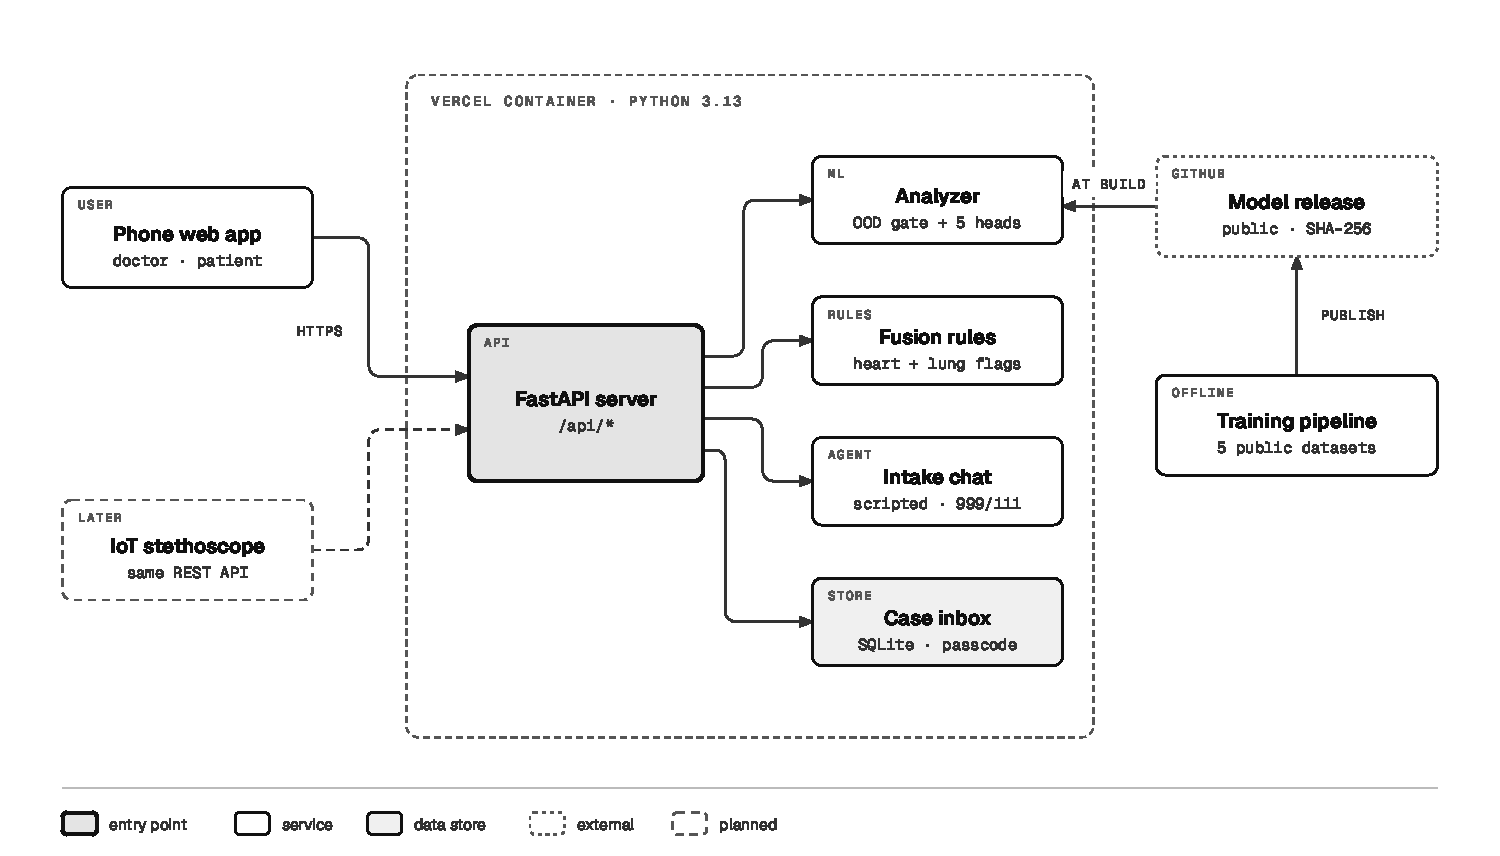
\includegraphics[width=0.92\textwidth]{fig-architecture.pdf}
\caption{System architecture. The phone app and any future stethoscope use the same REST API. Models are trained offline and published as a pinned release.}
\label{fig:arch}
\end{figure*}

\subsection{How the app is used}
The landing page explains the system with an animated heart and lungs drawn in WebGL, an interactive architecture diagram and a confidence-gauge figure, and then hosts the app itself in three tabs. In \emph{Analyse}, the user picks a held-out dataset sample, uploads a file, or records with the phone microphone, for the heart, the lungs, or both. The result shows an overall status (normal, abnormal or inconclusive), one line per model with its label and confidence, the dataset each model was trained on, and any cross-system flags. In \emph{Chat}, a patient answers a short intake and sends a summary to the doctor. In \emph{Inbox}, the doctor enters a passcode and reads the cases, each with the patient's answers, the AI findings and an urgency level. Every screen states that the tool is a research prototype and not a medical device.

Files above 3.5~MB are re-encoded on the phone to 4~kHz mono WAV before upload, because the host rejects request bodies above about 4.5~MB and the models only use content below 2~kHz.

\subsection{API}
Table~\ref{tab:api} lists the endpoints. Interactive documentation is generated at \texttt{/docs}. A future IoT stethoscope only needs to post audio to the analyse endpoints, so the hardware can be added without changing the server.

\begin{table}[t]
\caption{REST endpoints}
\label{tab:api}
\centering
\footnotesize
\begin{tabular}{@{}ll@{}}
\toprule
Endpoint & Purpose \\
\midrule
\texttt{POST /api/analyze/\{heart|lung\}} & analyse one recording \\
\texttt{POST /api/analyze/combined} & heart and lung, fused report \\
\texttt{GET /api/samples} & held-out dataset samples \\
\texttt{POST /api/chat} & next intake message \\
\texttt{POST /api/cases/from-chat} & send summary to inbox \\
\texttt{GET /api/cases} & doctor inbox (passcode) \\
\texttt{GET /api/health} & liveness and loaded models \\
\bottomrule
\end{tabular}
\end{table}

\section{Signal Processing and Models}

\subsection{Analysis of one recording}
Fig.~\ref{fig:flow} shows what happens to each recording. The audio is decoded (with ffmpeg as a fallback for phone formats), converted to mono at 4~kHz, and cut to the first 120~s. Recordings shorter than 2~s, containing invalid values, nearly silent, or clipped are rejected with a message that tells the user what to fix. A recording counts as clipped when more than 10\% of its samples sit in flat runs at the peak; this threshold rejects 2.3\% of ICBHI, against 19\% at a 1\% threshold. A fourth-order Butterworth band-pass then keeps 25 to 400~Hz for the heart and 50 to 1{,}900~Hz for the lungs.

\begin{figure}[t]
\centering
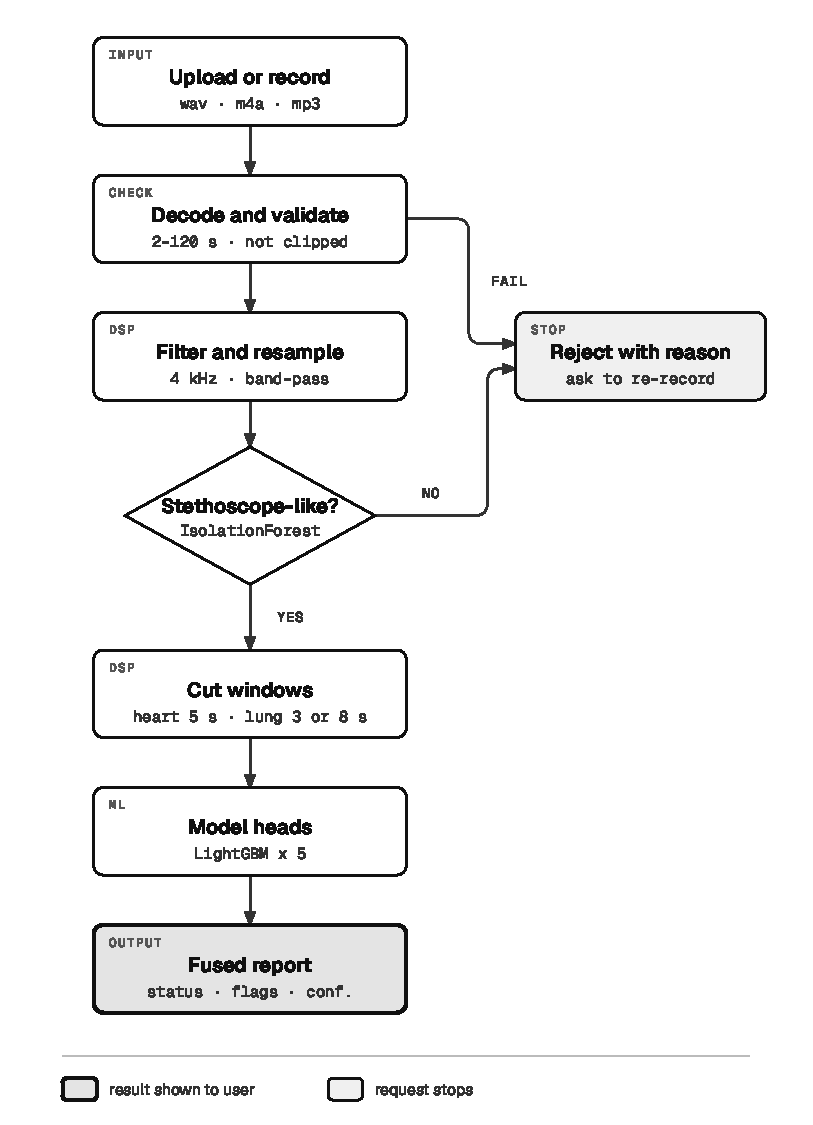
\includegraphics[width=0.86\columnwidth]{fig-flow.pdf}
\caption{Processing of one recording. Failed checks stop the request with a reason the user can act on.}
\label{fig:flow}
\end{figure}

An Isolation Forest \cite{liu2008} trained on features of real recordings then decides whether the input looks like stethoscope audio; its threshold allows 0.2\% false rejections on training data. It reliably rejects pure tones and speech-like signals. Band-limited white noise still passes, which is a known gap.

Accepted audio is cut into windows: 5~s with 2.5~s hop for heart models, 8~s with 4~s hop for lung diagnosis, and 3~s with 1.5~s hop for the lung sound model, which was trained on single breath cycles. Window probabilities are averaged per recording.

\subsection{Features and classifiers}
Each window is described by 40 MFCCs and their deltas, five spectral descriptors (centroid, bandwidth, roll-off, flatness, zero-crossing rate), each summarised by mean, standard deviation and skewness, plus relative energy in fixed frequency bands. Heart windows also get two envelope periodicity features that capture the regularity of the cardiac cycle. All features are computed with librosa \cite{mcfee2015}.

Each task uses a LightGBM gradient-boosted tree model \cite{ke2017} with 400 trees, learning rate 0.05, balanced class weights and row and column subsampling. For the two binary heart tasks, the decision threshold is chosen to maximise MAcc on out-of-fold predictions from five-fold patient-grouped cross-validation of the training set, so the test set never influences it. Fig.~\ref{fig:train} summarises the training pipeline, implemented with scikit-learn \cite{pedregosa2011}.

\begin{figure*}[t]
\centering
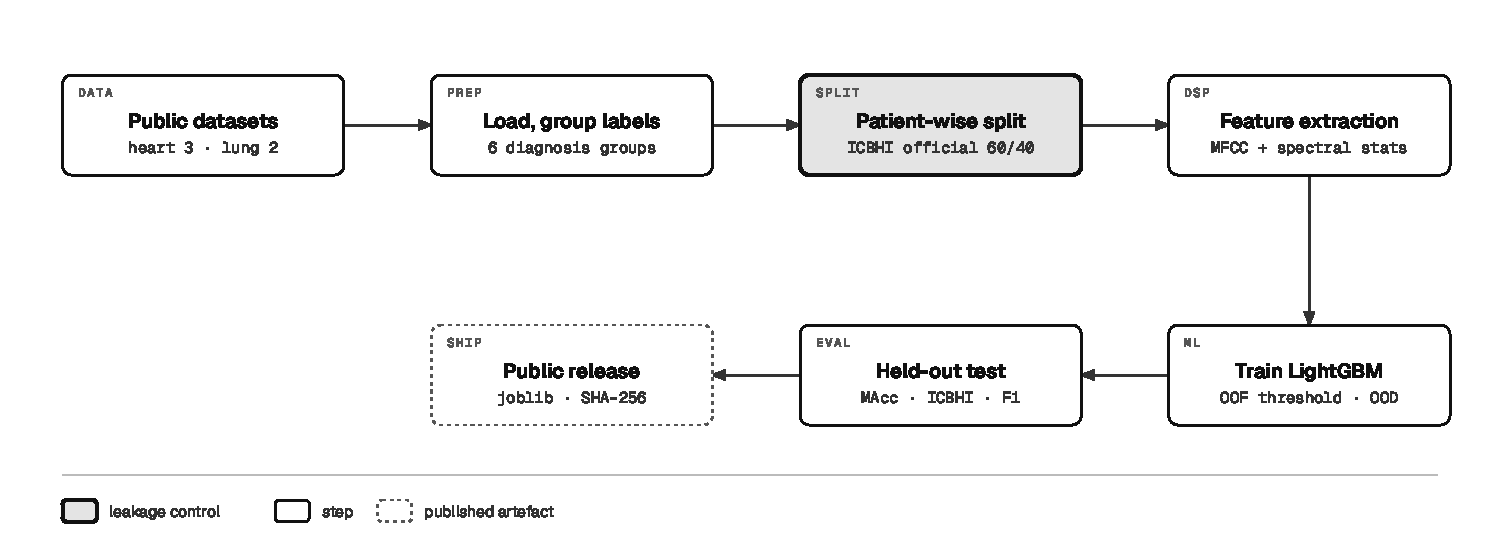
\includegraphics[width=0.86\textwidth]{fig-training.pdf}
\caption{Training and evaluation pipeline. The patient-wise split comes before any feature or threshold is fitted, which prevents leakage between training and test patients.}
\label{fig:train}
\end{figure*}

The five deployed heads are: heart normal/abnormal (CinC 2016), heart murmur present/absent (CirCor), heart valve class (Yaseen), lung sound per breath cycle (ICBHI: normal, crackle, wheeze, both) and lung diagnosis per recording (ICBHI and KAUH grouped into healthy, COPD, asthma, heart failure, infection and other).

\subsection{Combining heart and lung results}
No public dataset pairs heart and lung recordings from the same patient at a useful scale, so no joint model was trained. Each head runs on its own input and a rule layer merges them (Table~\ref{tab:rules}). The overall status is abnormal if any head predicts a non-normal class with confidence of at least 0.6, normal if every head predicts a normal class with that confidence, and inconclusive otherwise. Each flag names its rule so a clinician can check the reasoning.

\begin{table}[t]
\caption{Fusion rules}
\label{tab:rules}
\centering
\footnotesize
\begin{tabular}{@{}p{0.36\columnwidth}p{0.54\columnwidth}@{}}
\toprule
Condition & Flag shown \\
\midrule
Murmur or abnormal heart sound, and crackles & consider heart failure or fluid overload \\
Normal heart, and wheeze & airway disease pattern (e.g.\ asthma, COPD) \\
Any head low confidence & re-record in a quiet room \\
\bottomrule
\end{tabular}
\end{table}

\section{Patient Intake and Doctor Handoff}
Fig.~\ref{fig:seq} shows the patient-to-doctor flow. The patient first runs an analysis, then answers four questions in the chat: how long the symptoms have lasted, smoking history, previous heart or lung conditions, and current medicines. Every message is checked against a list of emergency phrases (for example chest pain, cannot breathe, blue lips, coughing blood, fainting). A match stops the chat and tells the patient to call 999 or go to A\&E, or to call NHS 111 if unsure.

\begin{figure*}[t]
\centering
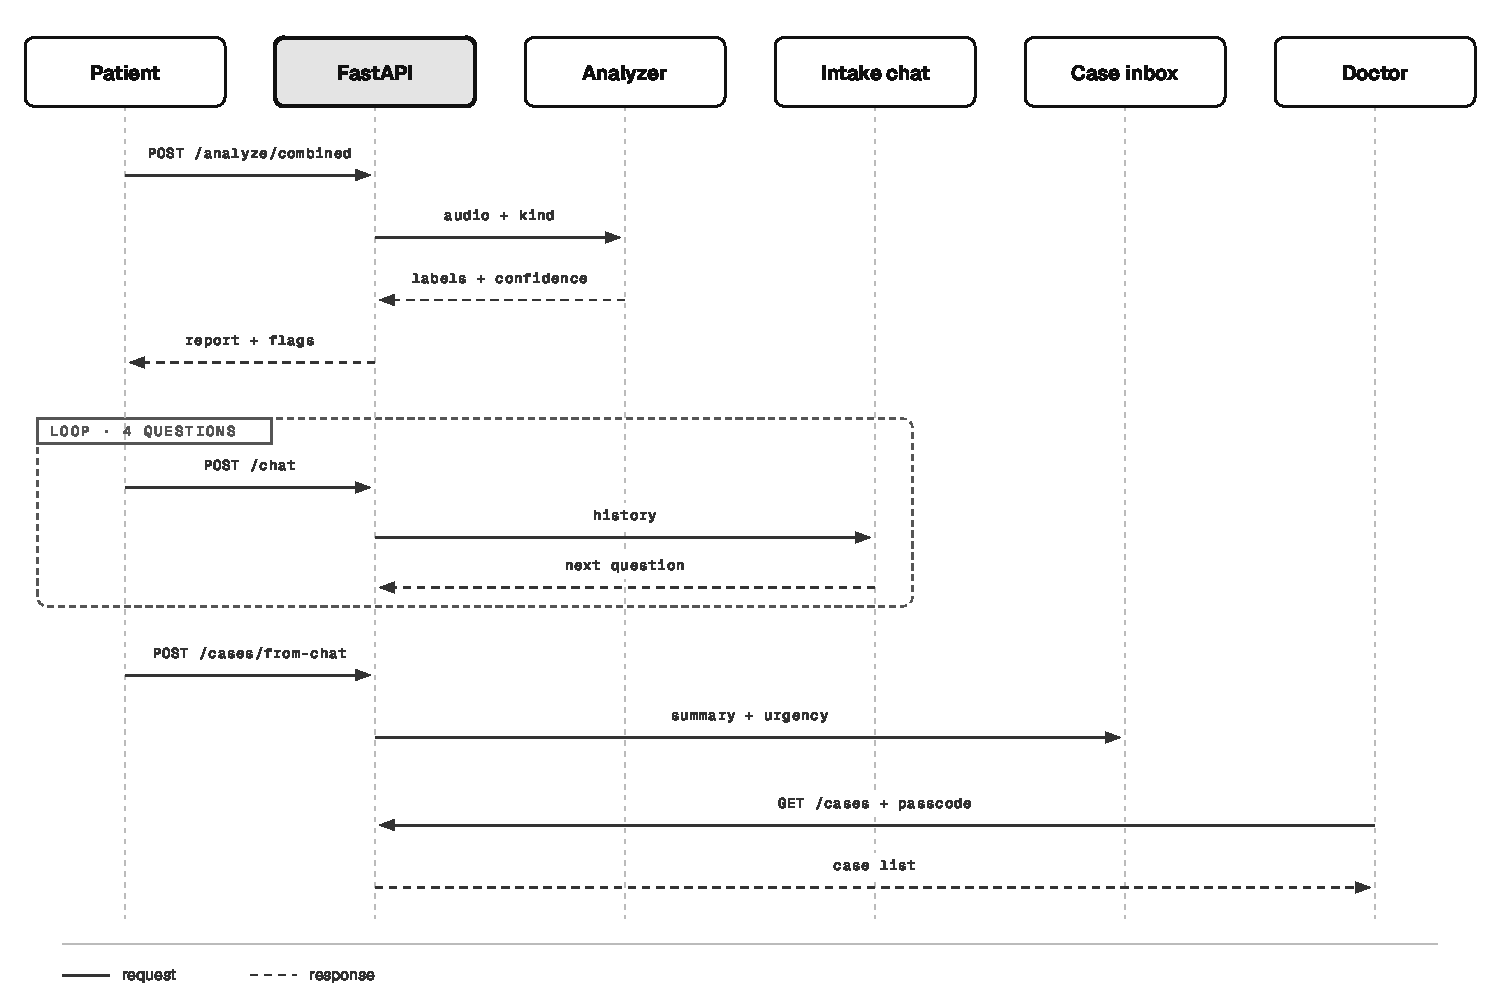
\includegraphics[width=0.86\textwidth]{fig-sequence.pdf}
\caption{Message sequence from patient analysis and intake to the doctor's inbox.}
\label{fig:seq}
\end{figure*}

When the intake finishes, the app builds a structured case with the symptoms, duration, history, AI findings and urgency (urgent after an emergency phrase, soon if the analysis is abnormal, routine otherwise) and stores it in SQLite. The doctor reads the inbox with a passcode set as a server secret and compared in constant time. Case creation is limited to 30 per hour per IP address.

The chat code can call a large language model through the Vercel AI Gateway or Groq when a key is configured. That route needs a payment card on file, so the deployed prototype uses the scripted intake, which costs nothing and behaves predictably. The safety rules apply in both modes: the assistant never diagnoses and never gives treatment advice.

\section{Implementation and Deployment}
The code is in Python 3.13 with pinned package versions and is public on GitHub. Training ran locally on an 8~GB Apple M3 laptop. The production image installs ffmpeg, fetches the source at a pinned commit and the model archive from the repository's release, verifies the archive's hash and starts uvicorn. All endpoints are synchronous so model inference does not block the event loop.

The test suite has 87 passing tests covering metrics, audio validation, dataset loaders, a training smoke test, the OOD gate, fusion rules, inference (including the optional AST path), the API and the intake agent. A review before release led to several fixes: secure temporary files for phone formats, rejection of invalid and clipped audio, a duration cap, the inbox passcode, rate limiting, closing a header-spoofing route to the model gateway, and wider emergency phrase matching.

\section{Evaluation}

\subsection{Protocol}
Test sets were held out by patient where the dataset publishes patient identifiers (CirCor, ICBHI, KAUH). CinC 2016 and Yaseen publish none, so they were split by recording, which may make their scores optimistic. The headline metrics are MAcc (mean of sensitivity and specificity) for the binary heart tasks, accuracy for Yaseen, the ICBHI score (mean of sensitivity and specificity over abnormal classes) for lung sounds \cite{rocha2019}, and macro-F1 for lung diagnosis, because ICBHI is about 86\% COPD and accuracy would mostly measure that.

\subsection{Results}
Table~\ref{tab:results} gives the held-out results. Published figures are shown for context only, because they use different test sets.

\begin{table*}[t]
\caption{Held-out results. Published references use other test sets and are not directly comparable.}
\label{tab:results}
\centering
\footnotesize
\begin{tabular}{@{}lllcccl@{}}
\toprule
Task & Data & Metric & Score & Macro-F1 & Test rec. (patients) & Published reference \\
\midrule
Heart normal/abnormal & CinC 2016, adults & MAcc & 0.882 & 0.810 & 648 (648) & $\approx$0.86 MAcc, hidden test set \cite{potes2016} \\
Heart murmur & CirCor, children & MAcc & 0.724 & 0.689 & 602 (175) & challenge winners, different metric \cite{reyna2023} \\
Heart valve class & Yaseen & Accuracy & 1.000 & 1.000 & 200 (200) & $\approx$0.97 \cite{yaseen2018} \\
Lung sound (4 class) & ICBHI official split & ICBHI score & 0.507 & 0.370 & 2{,}756 cycles (49) & $\approx$0.60 to 0.65 \cite{bae2023} \\
Lung diagnosis (6 group) & ICBHI + KAUH & Macro-F1 & 0.433 & 0.433 & 252 (49) & no single benchmark \\
\bottomrule
\end{tabular}
\end{table*}

The adult heart model detects 124 of 133 abnormal recordings (sensitivity 0.93) while flagging 87 of 515 normal ones (specificity 0.83), a sensible trade-off for a screening aid. The murmur model finds 80 of 123 murmurs. The perfect Yaseen score most likely reflects near-duplicate clips in a small, clean, recording-split dataset and should not be read as real-world accuracy. The lung sound model is the weakest part: it has sensitivity 0.285 and specificity 0.730, and it rarely predicts the combined crackle-and-wheeze class. In lung diagnosis, COPD is recognised well (158 of 164), while heart failure (1 of 12) and the small classes are poor.

\subsection{Robustness}
The adult heart model applied to the children's CirCor recordings reaches an MAcc of only 0.491. This drop is expected given the different population and devices, and it shows why local validation on the target population and stethoscope is needed before any clinical use.

\subsection{Live check}
All 34 held-out samples offered by the deployed app were sent through the public API. 32 matched their dataset label (heart normal/abnormal 4/4, murmur 3/4, valve 7/7, lung diagnosis 18/19), with a median response time of 1.6~s.

\subsection{Attempts to improve the lung model}
\label{sec:lungexp}
Four alternatives were evaluated on the same test cycles (Table~\ref{tab:cnn}). One clipped recording is now rejected, leaving 2{,}732 cycles from 49 patients. Each model was chosen on held-out training patients and scored on the test set once.

An EfficientNet-B0 \cite{tan2019} with ImageNet weights \cite{deng2009} was fine-tuned on 128-band log-mel spectrograms of each breath cycle with SpecAugment-style masking \cite{park2019}, using PyTorch \cite{paszke2019}, for 12 epochs on the laptop CPU. A 50/50 average of the CNN and the deployed model, with the weight fixed before scoring, did no better.

The Audio Spectrogram Transformer \cite{gong2021}, pretrained on AudioSet \cite{gemmeke2017} and kept frozen, turned each cycle into mean-pooled token embeddings from three layers, and a logistic-regression head was trained on them. It gave the best score, 0.533, but needs about 2.3~s per window on the laptop CPU. Dynamic int8 quantisation cut that to 0.7~s but lost the gain (0.502). A slimmed version kept 8 of the 12 layers, read 4~s of audio instead of 10.24~s by cropping the positional embeddings in time, used per-channel int8 weights, and had its head trained on the int8 embeddings themselves. It runs in about 70~ms per window, is 59~MB, and scores 0.519.

\begin{table}[t]
\caption{Lung sound models on the ICBHI official test split (2{,}732 cycles, 49 patients). Time is CPU time per window on an Apple M3.}
\label{tab:cnn}
\centering
\footnotesize
\begin{tabular}{@{}lccccr@{}}
\toprule
Model & ICBHI & Se & Sp & F1 & ms \\
\midrule
LightGBM (deployed) & 0.508 & 0.288 & 0.729 & 0.372 & $\approx$1 \\
EfficientNet-B0 CNN & 0.510 & 0.418 & 0.601 & 0.383 & -- \\
50/50 CNN + LightGBM & 0.511 & 0.321 & 0.702 & 0.369 & -- \\
AST frozen, float32 & 0.533 & 0.504 & 0.561 & -- & 2{,}300 \\
AST frozen, int8 & 0.502 & 0.475 & 0.528 & -- & 700 \\
Slim AST, int8 & 0.519 & 0.497 & 0.540 & -- & 70 \\
\bottomrule
\end{tabular}
\end{table}

To judge whether these differences are real, the slim AST and the deployed model were compared with a paired bootstrap over test patients (1{,}000 resamples). The slim model's advantage was +0.007 on average, with a 95\% interval of $-0.046$ to $+0.055$, and it won in 63\% of resamples. With only 49 test patients the ICBHI score carries roughly $\pm$0.05 of uncertainty, so every lung model in Table~\ref{tab:cnn} is statistically level with the deployed one. The models differ mainly in balance: the AST variants find far more abnormal cycles and raise more false alarms. The smaller and faster LightGBM model therefore stays in production. The slim AST is published as an optional model that the server can load without code changes.

\section{Limitations and Safety}
The models were trained on research datasets recorded with specific stethoscopes, populations and labelling practices, and their accuracy will not transfer unchanged to new devices or NHS patients. Two heart datasets lack patient identifiers. The heart and lung models were never trained on the same patients, so the fusion rules are clinical heuristics, not learned relationships. The OOD gate misses band-limited noise. The ICBHI test set has only 49 patients, which limits how finely lung models can be compared. The case inbox lives in SQLite inside a stateless container, so cases are lost on restart, and the passcode is a single shared secret, which is acceptable for a demonstration but not for patient data. The system has no clinical safety case, no data protection impact assessment and no regulatory approval, and it must not be used for real patient decisions.

\section{Future Work and Roadmap}
\label{sec:future}
Fig.~\ref{fig:roadmap} shows how the prototype could grow into a product. Each stage depends on the one before it.

\begin{figure*}[t]
\centering
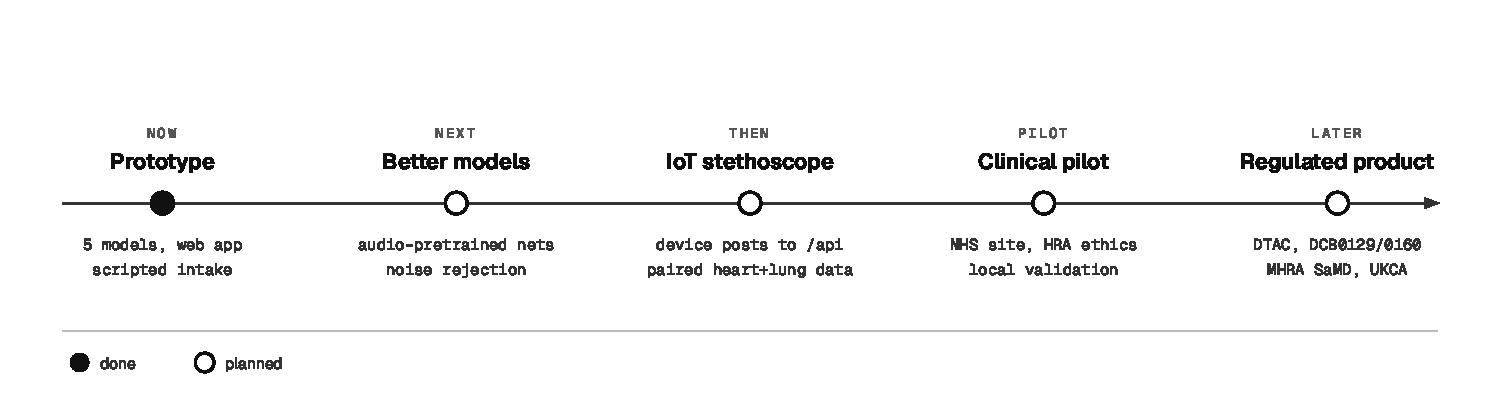
\includegraphics[width=0.86\textwidth]{fig-roadmap.pdf}
\caption{Roadmap from the current prototype to a regulated product.}
\label{fig:roadmap}
\end{figure*}

\subsection{Better models}
Frozen AST embeddings already match the best simple models here, and fine-tuning the whole transformer on a GPU, as in the Patch-Mix recipe \cite{bae2023}, is the likely route to the published 0.60 to 0.63. Respiratory foundation models such as OPERA \cite{zhang2024opera} and HeAR \cite{baur2024} are alternatives. A clear improvement should be shown with a confidence interval, ideally on more test patients than ICBHI's 49, for example by adding KAUH cycles. Heart sound segmentation \cite{springer2016} could improve the heart models. The OOD gate needs a dedicated stethoscope-versus-other classifier trained with noise, speech and environmental sounds as negatives, so that white noise is rejected. Confidence should also be calibrated so that the displayed percentages mean what they say.

\subsection{IoT stethoscope}
A digital stethoscope or a low-cost microphone module would stream or upload recordings to the existing analyse endpoints. Recording heart and lungs from the same patients would, for the first time, produce paired data from which a joint model could learn the cross-system patterns that the rules now approximate. The app would also need guidance on placement and recording length.

\subsection{Clinical pilot}
A pilot at an NHS site would need ethical approval through the Health Research Authority, a data protection impact assessment, and a prospective comparison against clinician auscultation and echocardiography or spirometry as reference standards. Results must be reported per device and per population. The infrastructure would move to UK-hosted servers with a managed database, individual clinician accounts, audit logs and encryption at rest. A language-model intake could replace the scripted one if it passes a safety evaluation.

\subsection{Regulated product}
Software that informs diagnosis is a medical device in the UK. The product would need clinical risk management under DCB0129 (manufacturer) and DCB0160 (deploying organisation), the NHS Digital Technology Assessment Criteria (DTAC), evidence matching the NICE Evidence Standards Framework \cite{nice2022}, and UKCA marking under the MHRA's software and AI as a medical device programme \cite{mhra2021}, most likely as Class IIa or higher.

\section{Conclusion}
The prototype shows that heart and lung sound analysis, a safety chain, a fused report and a patient-to-doctor handoff can be built and deployed with only public data and free infrastructure. The heart models are close to published results; the lung sound model is not, and four attempts to improve it, including an AudioSet transformer slimmed to run in 70~ms, gave gains within the noise of a 49-patient test set. The honest evaluation, the patient-wise splits and the documented failures give a solid base for the next steps: fine-tuned lung models, a real digital stethoscope, and a supervised pilot with NHS clinicians.

\section*{Availability}
Live demo: \url{https://auscultation-ai.vercel.app}. Source code, trained models (release \texttt{v5}) and the optional slim AST model (release \texttt{ast-slim-v1}) are public at \url{https://github.com/adityavdn/auscultation-ai}.

\begin{thebibliography}{30}

\bibitem{leng2015}
S. Leng, R. S. Tan, K. T. C. Chai, C. Wang, D. Ghista, and L. Zhong, ``The electronic stethoscope,'' \emph{BioMed. Eng. OnLine}, vol.~14, art.~66, 2015.

\bibitem{clifford2016}
G. D. Clifford \emph{et al.}, ``Classification of normal/abnormal heart sound recordings: The PhysioNet/Computing in Cardiology Challenge 2016,'' in \emph{Proc. Comput. Cardiol.}, vol.~43, 2016, pp.~609--612.

\bibitem{liu2016}
C. Liu \emph{et al.}, ``An open access database for the evaluation of heart sound algorithms,'' \emph{Physiol. Meas.}, vol.~37, no.~12, pp.~2181--2213, 2016.

\bibitem{goldberger2000}
A. L. Goldberger \emph{et al.}, ``PhysioBank, PhysioToolkit, and PhysioNet: Components of a new research resource for complex physiologic signals,'' \emph{Circulation}, vol.~101, no.~23, pp.~e215--e220, 2000.

\bibitem{oliveira2022}
J. Oliveira \emph{et al.}, ``The CirCor DigiScope dataset: From murmur detection to murmur classification,'' \emph{IEEE J. Biomed. Health Inform.}, vol.~26, no.~6, pp.~2524--2535, 2022.

\bibitem{reyna2023}
M. A. Reyna \emph{et al.}, ``Heart murmur detection from phonocardiogram recordings: The George B. Moody PhysioNet Challenge 2022,'' \emph{PLOS Digit. Health}, vol.~2, no.~9, art.~e0000324, 2023.

\bibitem{yaseen2018}
Yaseen, G.-Y. Son, and S. Kwon, ``Classification of heart sound signal using multiple features,'' \emph{Appl. Sci.}, vol.~8, no.~12, art.~2344, 2018.

\bibitem{rocha2018}
B. M. Rocha \emph{et al.}, ``A respiratory sound database for the development of automated classification,'' in \emph{Precision Medicine Powered by pHealth and Connected Health (ICBHI 2017)}, IFMBE Proc., vol.~66. Singapore: Springer, 2018, pp.~33--37.

\bibitem{rocha2019}
B. M. Rocha \emph{et al.}, ``An open access database for the evaluation of respiratory sound classification algorithms,'' \emph{Physiol. Meas.}, vol.~40, no.~3, art.~035001, 2019.

\bibitem{fraiwan2021}
M. Fraiwan, L. Fraiwan, B. Khassawneh, and A. Ibnian, ``A dataset of lung sounds recorded from the chest wall using an electronic stethoscope,'' \emph{Data in Brief}, vol.~35, art.~106913, 2021.

\bibitem{zhang2024opera}
Y. Zhang \emph{et al.}, ``Towards open respiratory acoustic foundation models: Pretraining and benchmarking,'' in \emph{Adv. Neural Inf. Process. Syst. (Datasets and Benchmarks Track)}, 2024.

\bibitem{potes2016}
C. Potes, S. Parvaneh, A. Rahman, and B. Conroy, ``Ensemble of feature-based and deep learning-based classifiers for detection of abnormal heart sounds,'' in \emph{Proc. Comput. Cardiol.}, vol.~43, 2016, pp.~621--624.

\bibitem{springer2016}
D. B. Springer, L. Tarassenko, and G. D. Clifford, ``Logistic regression-HSMM-based heart sound segmentation,'' \emph{IEEE Trans. Biomed. Eng.}, vol.~63, no.~4, pp.~822--832, 2016.

\bibitem{gong2021}
Y. Gong, Y.-A. Chung, and J. Glass, ``AST: Audio spectrogram transformer,'' in \emph{Proc. Interspeech}, 2021, pp.~571--575.

\bibitem{gemmeke2017}
J. F. Gemmeke \emph{et al.}, ``Audio Set: An ontology and human-labeled dataset for audio events,'' in \emph{Proc. IEEE ICASSP}, 2017, pp.~776--780.

\bibitem{bae2023}
S. Bae \emph{et al.}, ``Patch-mix contrastive learning with audio spectrogram transformer on respiratory sound classification,'' in \emph{Proc. Interspeech}, 2023, pp.~5436--5440.

\bibitem{kong2020}
Q. Kong, Y. Cao, T. Iqbal, Y. Wang, W. Wang, and M. D. Plumbley, ``PANNs: Large-scale pretrained audio neural networks for audio pattern recognition,'' \emph{IEEE/ACM Trans. Audio, Speech, Lang. Process.}, vol.~28, pp.~2880--2894, 2020.

\bibitem{baur2024}
S. Baur \emph{et al.}, ``HeAR: Health acoustic representations,'' arXiv:2403.02522, 2024.

\bibitem{liu2008}
F. T. Liu, K. M. Ting, and Z.-H. Zhou, ``Isolation forest,'' in \emph{Proc. IEEE Int. Conf. Data Mining (ICDM)}, 2008, pp.~413--422.

\bibitem{mcfee2015}
B. McFee \emph{et al.}, ``librosa: Audio and music signal analysis in Python,'' in \emph{Proc. 14th Python in Science Conf.}, 2015, pp.~18--25.

\bibitem{ke2017}
G. Ke \emph{et al.}, ``LightGBM: A highly efficient gradient boosting decision tree,'' in \emph{Adv. Neural Inf. Process. Syst.}, vol.~30, 2017, pp.~3146--3154.

\bibitem{pedregosa2011}
F. Pedregosa \emph{et al.}, ``Scikit-learn: Machine learning in Python,'' \emph{J. Mach. Learn. Res.}, vol.~12, pp.~2825--2830, 2011.

\bibitem{tan2019}
M. Tan and Q. V. Le, ``EfficientNet: Rethinking model scaling for convolutional neural networks,'' in \emph{Proc. Int. Conf. Mach. Learn. (ICML)}, 2019, pp.~6105--6114.

\bibitem{deng2009}
J. Deng, W. Dong, R. Socher, L.-J. Li, K. Li, and L. Fei-Fei, ``ImageNet: A large-scale hierarchical image database,'' in \emph{Proc. IEEE CVPR}, 2009, pp.~248--255.

\bibitem{park2019}
D. S. Park \emph{et al.}, ``SpecAugment: A simple data augmentation method for automatic speech recognition,'' in \emph{Proc. Interspeech}, 2019, pp.~2613--2617.

\bibitem{paszke2019}
A. Paszke \emph{et al.}, ``PyTorch: An imperative style, high-performance deep learning library,'' in \emph{Adv. Neural Inf. Process. Syst.}, vol.~32, 2019, pp.~8024--8035.

\bibitem{nice2022}
National Institute for Health and Care Excellence, ``Evidence standards framework for digital health technologies,'' NICE, London, U.K., 2022.

\bibitem{mhra2021}
Medicines and Healthcare products Regulatory Agency, ``Software and AI as a medical device change programme,'' MHRA, London, U.K., 2021.

\end{thebibliography}

\end{document}
